\FloatBarrier
\section{Communication}

\subsection{The External Bus Interface}
The microcontroller communicates with the FPGA design using the External Bus
Interface (EBI) of the Giant Gecko microcontroller. The EBI is a parallel bus
with a separate data and address bus in addition to the chip select and read and
write enable signals, all active low\cite{efm_ebi}.

The communication between the MCU and the FPGA uses 23 address lines and 16
data lines. All transfers are initiated by the chip select signal going low.
Then, for write transfers, the data and address lines are set up and the
write enable signal is asserted, see figure \ref{fig:ebi_write}. For reads,
the address is set up and the data line is put in high impedance mode before
the read enable signal is asserted, see figure \ref{fig:ebi_read}.

\begin{figure}[h]
	\centering
	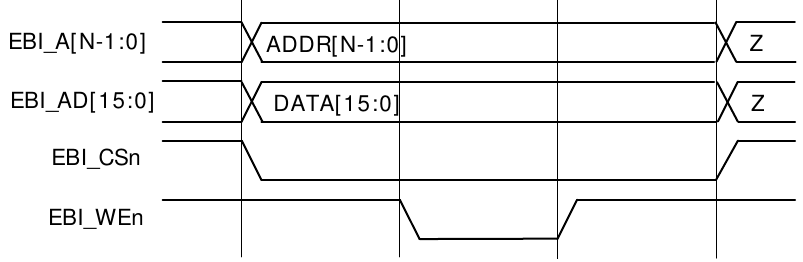
\includegraphics[width=0.8\linewidth]{figures/fpga/ebi_write.png}
	\caption{EBI write transfer\cite[p.6]{efm_ebi}}
	\label{fig:ebi_write}
\end{figure}



\begin{figure}[h]
	\centering
	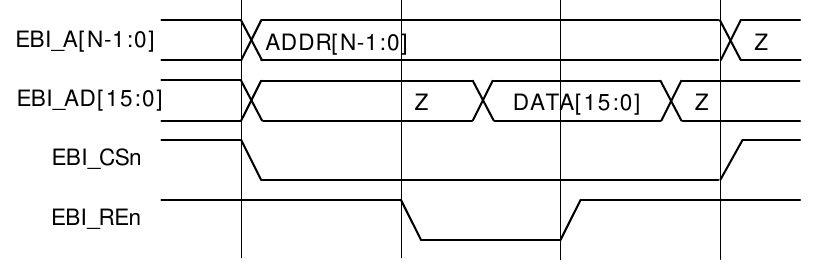
\includegraphics[width=0.8\linewidth]{figures/fpga/ebi_read.png}
	\caption{EBI read transfer\cite[p.7]{efm_ebi}}
	\label{fig:ebi_read}
\end{figure}



\FloatBarrier
\subsection{The Internal Bus}

The internal bus is used to transfer data to and from modules in the FPGA.
All transfers are initiated by the microcontroller on the EBI bus, and the
EBI controller module translates between the EBI and the internal bus.

\subsubsection{The EBI controller}
The EBI controller module is used to handle EBI transfers initiated by the
microcontroller. It consists of a simple state machine, illustrated in
figure \ref{fig:ebi_ctrl_fsm}. When an EBI transfer is executed, the
internal bus, described in is used to store or retrieve data from a module
in the FPGA.

In the idle state, the EBI data lines are set as high impedance, which
causes the microcontroller to have control of the data bus. Only when
a value is read over the EBI bus, does the EBI controller take control of
the data lines.

To save power, a clock gate is used to turn off the functional clock to
the EBI controller when the chip select signal is deasserted.

\begin{figure}[h]
	\centering
	% TODO: Make the arrows in separate directions be separate arrows
	\begin{tikzpicture}[shorten >= 1pt,node distance=2cm,on grid,auto]
		\node[state,initial] (idle) {idle};
		\node[state] (read) [above right=of idle] {read};
		\node[state] (write) [below right=of idle] {write};
		\path[->]
			(idle) edge node {\small RE = 0} (read)
			       edge node [swap] {\small EW = 0} (write)
			(read) edge node {\small RE = 1} (idle)
			(write) edge node [swap] {\small WE = 1} (idle);
	\end{tikzpicture}
	\caption{EBI controller state machine}
	\label{fig:ebi_ctrl_fsm}
\end{figure}




\subsubsection{Addressing}

Modules in the FPGA is addressed using a simple hierarchical scheme, where the
address is divided into three parts; the pipeline where the module is located,
the ``index'' of the module and an address specifying where in the module to
read or write data. Figure \ref{fig:ebi_addresses} illustrates the address
format.

\begin{figure}[H]
	\centering
	\begin{bytefield}[endianness=big,bitwidth=0.04\linewidth]{23}
		\bitheader{0-22}\\
		\bitbox{1}{T} &
		\bitbox{2}{\tiny Pipeline} &
		\bitbox{4}{Device} &
		\bitbox{2}{\tiny Subdev} &
		\bitbox{14}{Address}
	\end{bytefield}
	\caption{FPGA address format}
	\label{fig:ebi_addresses}
\end{figure}




\FloatBarrier
\subsubsection{Read Transfers}

A read transfer is initiated when the read enable line from the microcontroller goes low.
The EBI controller sets up the internal address signals and asserts the internal read enable
signal. This causes the requested data to be available in the next clock cycle. The EBI
controller switches to read state, where it remains until the read enable signal is deasserted.

\subsubsection{Write Transfers}

Write transfers are initiated the same way as read transfers. As the write-enable signal goes
low, the destination address is latched into the internal address bus and the internal data
lines are set to the value of the EBI data lines. The internal write enable signal is asserted
and the EBI controller enters the write state. In the write state the internal write enable
signal is reset, and when the EBI write enable signal is deasserted, idle mode is reentered.

